% -*- root: ../main.tex -*-

% Devono essere esposte le scelte progettuali operate nelle varie fasi di sviluppo dell'elaborato. In questa sezione devono essere documentati gli schemi di progetto relativamente all'architettura complessiva del sistema e alle sue componenti di rilievo che possano meritare un'analisi di dettaglio. Per le componenti software si può ricorrere ad esempio a diagrammi delle classi, di sequenza, stato, attività. Per le componenti hardware è possibile includere opportuni schemi in grado di descrivere l'architettura fisica adottata.
% 15000 - 24000 battute (comprende anche capitolo Design)

\chapter{Design Architetturale}
    Dopo un intenso periodo di Domain Driven Design, si è passati si è proceduto alla fase di Design Architetturale, agevolata di molto da quest'ultimo. Infatti da un confronto mirato con il cliente l'architettura ottimale è emersa quasi naturalmente. Lasciando spazio alla definizione dei dettagli più tecnici che riportiamo in seguito.
    \section{Architettura Generale}
    L'architettura generale del sistema è stata concepita in due macro aree: la parte IoT [Fig. \ref{fig:DesignArchitettura}. in alto] e la parte cloud [Fig. \ref{fig:DesignArchitettura}. in basso]. Le due sfruttano la connessione internet per connettersi, lo scambio di messaggi avviene attraverso il protocollo MQTT, mentre il flusso video viene passato per mezzo del protocollo RTSP. 
    
    Il sistema IoT risiede su una rete privata e comunica all'esterno per mezzo di questi due protocolli. Le parti salienti sono la sensoristica che fornisce le informaioni sull'ambiente circostante al microcontrollore, il quale le elabora e utilizza gli attuatori in base alle informazioni ricavate sia dai sensori che dal cloud.
    
    La parte cloud si interfaccia per mezzo dell'applicativo IOT Core ai sensori, i messaggi MQTT vengono elaborati da AWS Lambda e, qualora opportuno, immagazzinati come dati nel database. L'applicativo web, hostato su AWS Amplify, si interfaccia anch'esso con AWS Lambda, passando per Amazon API Gateway. Questo sia per recuperare i dati dal database DynamoDB e mostrare le statistiche, che per diramare il cambio dei settaggi fino ai microcontrollori. Infine, l'applicativo si occupa anche di mostrare il flusso video proveniente dalla board per le telecamere di sorveglianza. 
    %immagine architettura generale
    \begin{figure}[H]
        \caption{Design dell'architettura generale del sistema}
        \label{fig:DesignArchitettura}
        \centering
       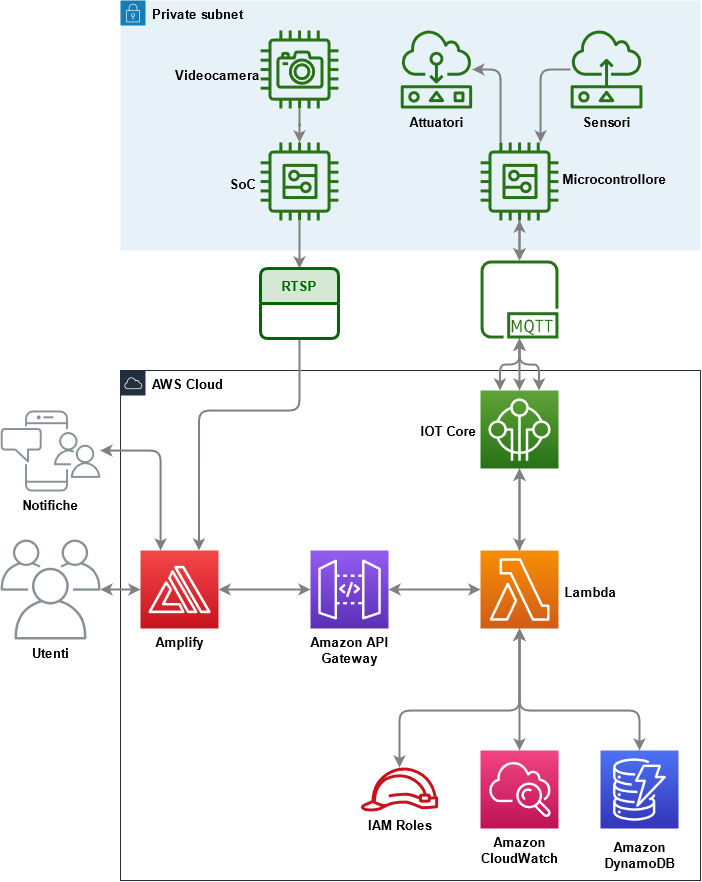
\includegraphics[width=0.8\textwidth]{DrawIo/Architecture.png}
    \end{figure}
    
    \section{Scelte Tecnologiche Cruciali}
        \subsection{AWS}
        Tra i servizi messi a disposizione da AWS vi è anche Amazon Cognito che permette di gestire gli utenti. 
        E' stato valutato Amazon Cognito ma è stato scartato perché gli utenti sono troppo pochi.
        
        \subsection{Protocolli di comunicazione}
        \subsubsection{Scambio messaggi}
        Come protocolli di comunicazione sono stati considerati i principali protocolli per la comunicazione IoT. Tra quelli di livello applicazione: 
        \begin{itemize}
            \item \textbf{AMQP (Advanced Message Queuing Protocol)}, protocollo che consente a un'ampia gamma di sistemi e applicazioni di interagire, creando messaggistica standardizzata su scala industriale.
            \item \textbf{CoAP (Constrained Application Protocol)}, protocollo adatto alle limitazioni di larghezza di banda e di rete, per dispositivi con capacità limitata, ma prevalentemente per la connessione nelle comunicazioni da computer a computer. 
            \item \textbf{DDS (Data Distribution Service)}, protocollo per comunicazioni peer-to-peer. In generale semplifica la distribuzione, incrementa l'affidabilità e riduce la complessità.
            \item \textbf{MQTT (Message Queue Telemetry Transport)}, protocollo di messaggistica progettato per comunicazioni IoT. MQTT usa un criterio di tipo publish-subscribe ed è ideale per dispositivi di dimensioni ridotte che richiedono efficienza a livello di larghezza di banda e uso della batteria.
        \end{itemize}
        La scelta è ricaduta su MQTT per la sua leggerezza ed efficienza, per la possibilità di instaurare comunicazioni bidirezionali tra molti dispositivi. Il design inoltre è molto semplificato dalla possibilità di creare topic a cui iscriversi o in cui pubblicare i messaggi.
        
        \subsubsection{Streaming Video}
        Per lo streaming video sono stati considerate due opzioni: streaming attraverso RTSP e attraverso HTTP con un server e HTML5. 
        RTSP è di sicuro la scelta più popolare perché adottato come protocollo dalle IP-cam e telecamere di sorveglianza. Nonostante ciò non è compatibile con HTTP e, non potendo fare lo stream su HTTP direttamente, non è visualizzabile nativamente dai browser. Questo protocollo è infatti usato internamente alle reti private. Volendo esporre il flusso video anche al di fuori della rete privata del committente la scelta è ricaduta sulla seconda opzione. Inoltre, con questa tecnologia alla videosorveglianza si ha accesso con qualsiasi browser, da computer o da smartphone.
        
        \subsection{Microcontrollori e Soc}
        \subsubsection{Hardware}
        Le piattaforme di sviluppo per l'IoT tenute presente sono state molteplici, da board con potenza computazionale più elevata, come Raspberry Pi, a scendere fino a ESP e le varianti Arduino. 
        
        Le board Arduino sono state scartate quasi subito, per la poca potenza computazionale e la necessità di moduli aggiuntivi per le connessioni. 
        La board RaspBerry Pi è stata scelta per task più computazionalmente onerosi, legati alla gestione ambientale, quali la video sorveglianza e l'analisi immagini. 
        Questa scelta non può essere invece adottata per la gestione delle gabbie. Le principali motivazioni risiedono nel fatto che il numero è variabile e il costo supererebbe molto superiore al budget. 
        La scelta in questo caso è ricaduta sull'ESP, non solo per il forte fattore cost-competitive, e per il supporto a Bluetooth e WiFi integrati, ma anche per il supporto della community e l'ottima potenza computazionale. Inoltre, rinunciando all'analisi immagini e alla qualità video a favore dei costi, il cliente potrà anche scegliere di sostituire la board Raspberry con un più economico ESP32-CAM.
        Con l'ESP8266 le prime settimane il lavoro di indagine preliminare ha rilevato qualche che risultava troppo limitato per utilizzare MicroPython.
        Tra ESP8266 e ESP32 è stato preferito quest'ultimo, anche per lasciare della capacità di calcolo per eventuali future espansioni e richieste del committente. 
        \subsubsection{Linguaggio di programmazione}
        Per quanto riguarda l'implementazione del codice nel microcontrollore, sono state presi in considerazione quattro scelte relative ai framework di sviluppo e ai linguaggi da adottare: 
        \begin{itemize}
            \item \textbf{C++} è il linguaggio attualmente più diffuso nell'ambito. 
            \item \textbf{Node-RED} è un tool di programmazione flow-based basato su browser, sviluppato su NodeJs e programmabile in JavaScript.
            \item \textbf{MicroPython} è un porting più leggero del compilatore Python3, eseguibile direttamente su microcontrollori. Include le principali librerie di Python e moduli aggiuntivi per l'accesso all'hardware di basso livello.
            \item \textbf{Espruino} è un interprete JavaScript open-source per microcontrollori. E' stato progettato per unità con poca RAM.
        \end{itemize}
        Sicuramente il più performante e con più librerie è C, ma risulta anche difficilmente testabile e pone challange non indifferenti per la configurazione dei sensori e per lo sviluppo di programmi molto complessi. Node-RED, basato su Node.js, ha il pieno vantaggio del suo modello non bloccante e event-driven. MicroPython d'altra parte offre un modello ad oggetti, testabile, sia semplice che elastico, con una buona base di librerie. Infine, Espruino, interprete JavaScript anch'esso, di facile utilizzo e dall'interfaccia semplificata. 
        I fattori chiave che il team ha preso in considerazione per la scelta sono stati: 
        \begin{itemize}
            \item la potenza espressiva rapportata alla chiarezza del linguaggio. 
            \item la testabilità del codice
            \item il numero di librerie e la futura possibilità di estensione del progetto.
        \end{itemize}
        Alla luce delle considerazioni fatte, si è scelto \textbf{MicroPython} per lo sviluppo, il testing e l'automatizzazione nei microcontrollori. Questo permette di allinearsi con l'utilizzo di \textbf{Pyhton} per il Raspberry.

    \section{Pattern Architetturali Utilizzati}
        \subsection{Client-Server}
        L'utilizzo del pattern client-server, nella videosorveglianza, ha permesso di esporre il flusso video su un server apposito e di accederci da qualunque dispositivo dotato di connessione. 
    
        \subsection{Pusblish-Subscribe}
        L'utilizzo del pattern publish-subscribe, è stata una scelta chiave per la modularità del sistema. La divisione in topic ha portato un maggiore ordine e una modellazione più vicina al vero dominio. 
        
        \subsection{Master-Slave}
        E' stato fatto uso dell'architettura master-slave per la gestione dei microcontrollori. Questa permette di espanderne il numero a piacimento, mandando istruzioni specifiche o generali per controllarne il comportamento.
        
        \subsection{Scheduling Cooperativo}
        Nei sistemi embedded è stato adottato lo scheduling cooperativo per evitare tante pitfall dello scheduling preemptive, quali l'interruzione di un processo di misura Real Time, quale quello della chiusura della valvola dell'acqua o la misura del battito cardiaco.
        
        \subsection{State Machine}
        Per definire il comportamento dei microcontrollori in maniera chiara è stata usata la modellazione con macchine a stati. Questa ha permesso di ridurre la probabilità di bug nel software e di isolare i componenti permettendo una futura espansione del comportamento. 